\documentclass[xcolor=dvipsnames]{beamer}

\usepackage[utf8]{inputenc}
\usepackage[T1]{fontenc}
\usepackage[french]{babel}
\usepackage[babel=true]{csquotes}
\frenchbsetup{StandardLists=true}
\usepackage{graphicx}
\usepackage{color}
\usepackage{hyperref}
\usepackage{float}
\usepackage{pifont}
\usepackage{enumitem}
\hypersetup{colorlinks,linkcolor=,urlcolor=blue}
\mode<presentation>
%\definecolor{color_primary}{rgb}{0.827, 0.541, 0.211}
%\usecolortheme[named=color_primary]{structure}
{
%\usetheme{Bergen}
%\usetheme{Boadilla}
\usetheme{Madrid}
%\usetheme{AnnArbor}
%\usetheme{CambridgeUS}
%\usetheme{EastLansing}
%\usetheme{Rochester}
%\usetheme{Montpellier}
%\usetheme{Berkeley}
%\usetheme{Darmstadt}
%\usetheme{Frankfurt}

\definecolor{color_primary}{rgb}{0.827, 0.541, 0.211}
\definecolor{color_secondary}{rgb}{0.976, 0.780, 0.541}
\setbeamercolor{frametitle}{bg=color_primary}
\setbeamercolor{titlelike}{bg=color_primary}


%\setbeamercolor{title}{bg=NASAblue, fg=white} % title block on first slide
\setbeamercolor{palette primary}{bg=color_primary, fg=white} %right-hand side of bottom
\setbeamercolor{palette secondary}{bg=color_secondary, fg=white} % center bottom
\setbeamercolor{palette tertiary}{bg=color_primary,fg=white} % left bottom

\setbeamercovered{transparent}
}

\title[Dev. Mobiles]{Présentation d'un projet de développement d'application mobile :\\Soukouss Challenge}
\author{David~Boisedu et Alexandre~Boyer}
\institute[]{M1 Informatique}
\date{\today}


\AtBeginSection[]
{
  \begin{frame}
  %\frametitle{Sommaire}
  %\tableofcontents[currentsection, hideothersubsections, pausesubsections]
  \vfill
  \centering
  \begin{beamercolorbox}[sep=8pt,center,shadow=true,rounded=true]{title}
    \usebeamerfont{title}\insertsectionhead\par%
  \end{beamercolorbox}
  \vfill
  \end{frame} 
}

\setbeamersize{text margin left=1cm, text margin right=1cm}


\begin{document}
\logo{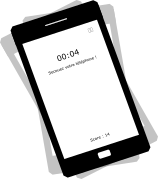
\includegraphics[height=10mm]{Images/g1354.png}}

\begin{frame}
    \titlepage
\end{frame}

\section{Introduction}

\begin{frame}{Idées principales}
    \begin{columns}[T]
     \begin{column}[c]{5cm}
        \begin{center}
\includegraphics[height=3cm]{Images/wall-clock.png}
        \end{center}
        \begin{center} Permet d'échapper à l'ennui
        \end{center}
     \end{column}
     \begin{column}[c]{5cm}
     \begin{center}
\includegraphics[height=3cm]{Images/hand_phone.png}
        \end{center}
        \begin{center} Facile à prendre en main
        \end{center}
     \end{column}
     \end{columns}
\end{frame}

\begin{frame}{Fonctionnalités requises}
    \begin{columns}[T]
     \begin{column}[c]{3cm}
        \begin{center}
\includegraphics[height=2cm]{Images/swipe.png}
        \end{center}
        \begin{center} Gestes courants
        \end{center}
     \end{column}
     \begin{column}[c]{3cm}
     \begin{center}
\includegraphics[height=2cm]{Images/shake.png}
        \end{center}
        \begin{center} Capteurs
        \end{center}
     \end{column}
     \begin{column}[c]{3cm}
     \begin{center}
\includegraphics[height=2cm]{Images/music-from-phone.png}
        \end{center}
        \begin{center} Audio
        \end{center}
     \end{column}
     \end{columns}
\end{frame}

\section{Objectifs du projet}

\begin{frame}{Objectif principal}
    \begin{columns}[T]
     \begin{column}[c]{5cm}
     \begin{center}
         \Large{Développer une application ludique qui utilise les capteurs du téléphone.}
     \end{center}
     \end{column}
     \begin{column}[c]{5cm}
          \begin{center}
\includegraphics[height=3cm]{Images/phone.png} \end{center}
     \end{column}
     \end{columns}
\end{frame}

\begin{frame}{Fonctions de l'application}
    \LARGE{Doit permettre à l'utilisateur de :}
    \vspace{2em}
    \begin{itemize}[label=\textbullet, font=\large \color{color_primary}]
        \Large{
        \item Jouer une partie
        \item D'afficher ses meilleurs scores
        \item De sauvegarder les scores
        }
    \end{itemize}
\end{frame}

\section{Réalisation}

\begin{frame}{Réalisation}
    \begin{columns}[T]
    \begin{column}[c]{5cm}
        \textbf{\Large{Environnement logiciel}}
        \vspace{2em}
        \begin{itemize}[label=\textbullet]
            \item Android Studio 
\includegraphics[height=0.5cm]{Images/1200px-Android_Studio_icon.svg.png}
            \item GitHub 
\includegraphics[height=0.5cm]{Images/1200px-Octicons-mark-github.svg.png}
            \item Inkscape 
\includegraphics[height=0.5cm]{Images/1200px-Inkscape_Logo.svg.png}
        \end{itemize}
    \end{column}
    \begin{column}[c]{5cm}
        \textbf{\Large{Autre plateformes utiles à la réalisation du projet}}
        \vspace{1em}
        \begin{itemize}[label=\textbullet]
            \item Moqups.com 
\includegraphics[height=0.5cm]{Images/moqups.png}
            \item Trello 
\includegraphics[height=0.5cm]{Images/logo_trello.png}
            \item Messenger 
\includegraphics[height=0.5cm]{Images/1200px-Facebook_Messenger_4_Logo.svg.png}
        \end{itemize}
    \end{column}
    \end{columns}
\end{frame}

\section{Description générale de l'application}

\begin{frame}{Description générale de l'application}
    \begin{columns}[T] 
     \begin{column}[c]{5cm}
     \LARGE{La vue d'accueil}
     \end{column}
     \begin{column}[c]{5cm}
        \begin{center}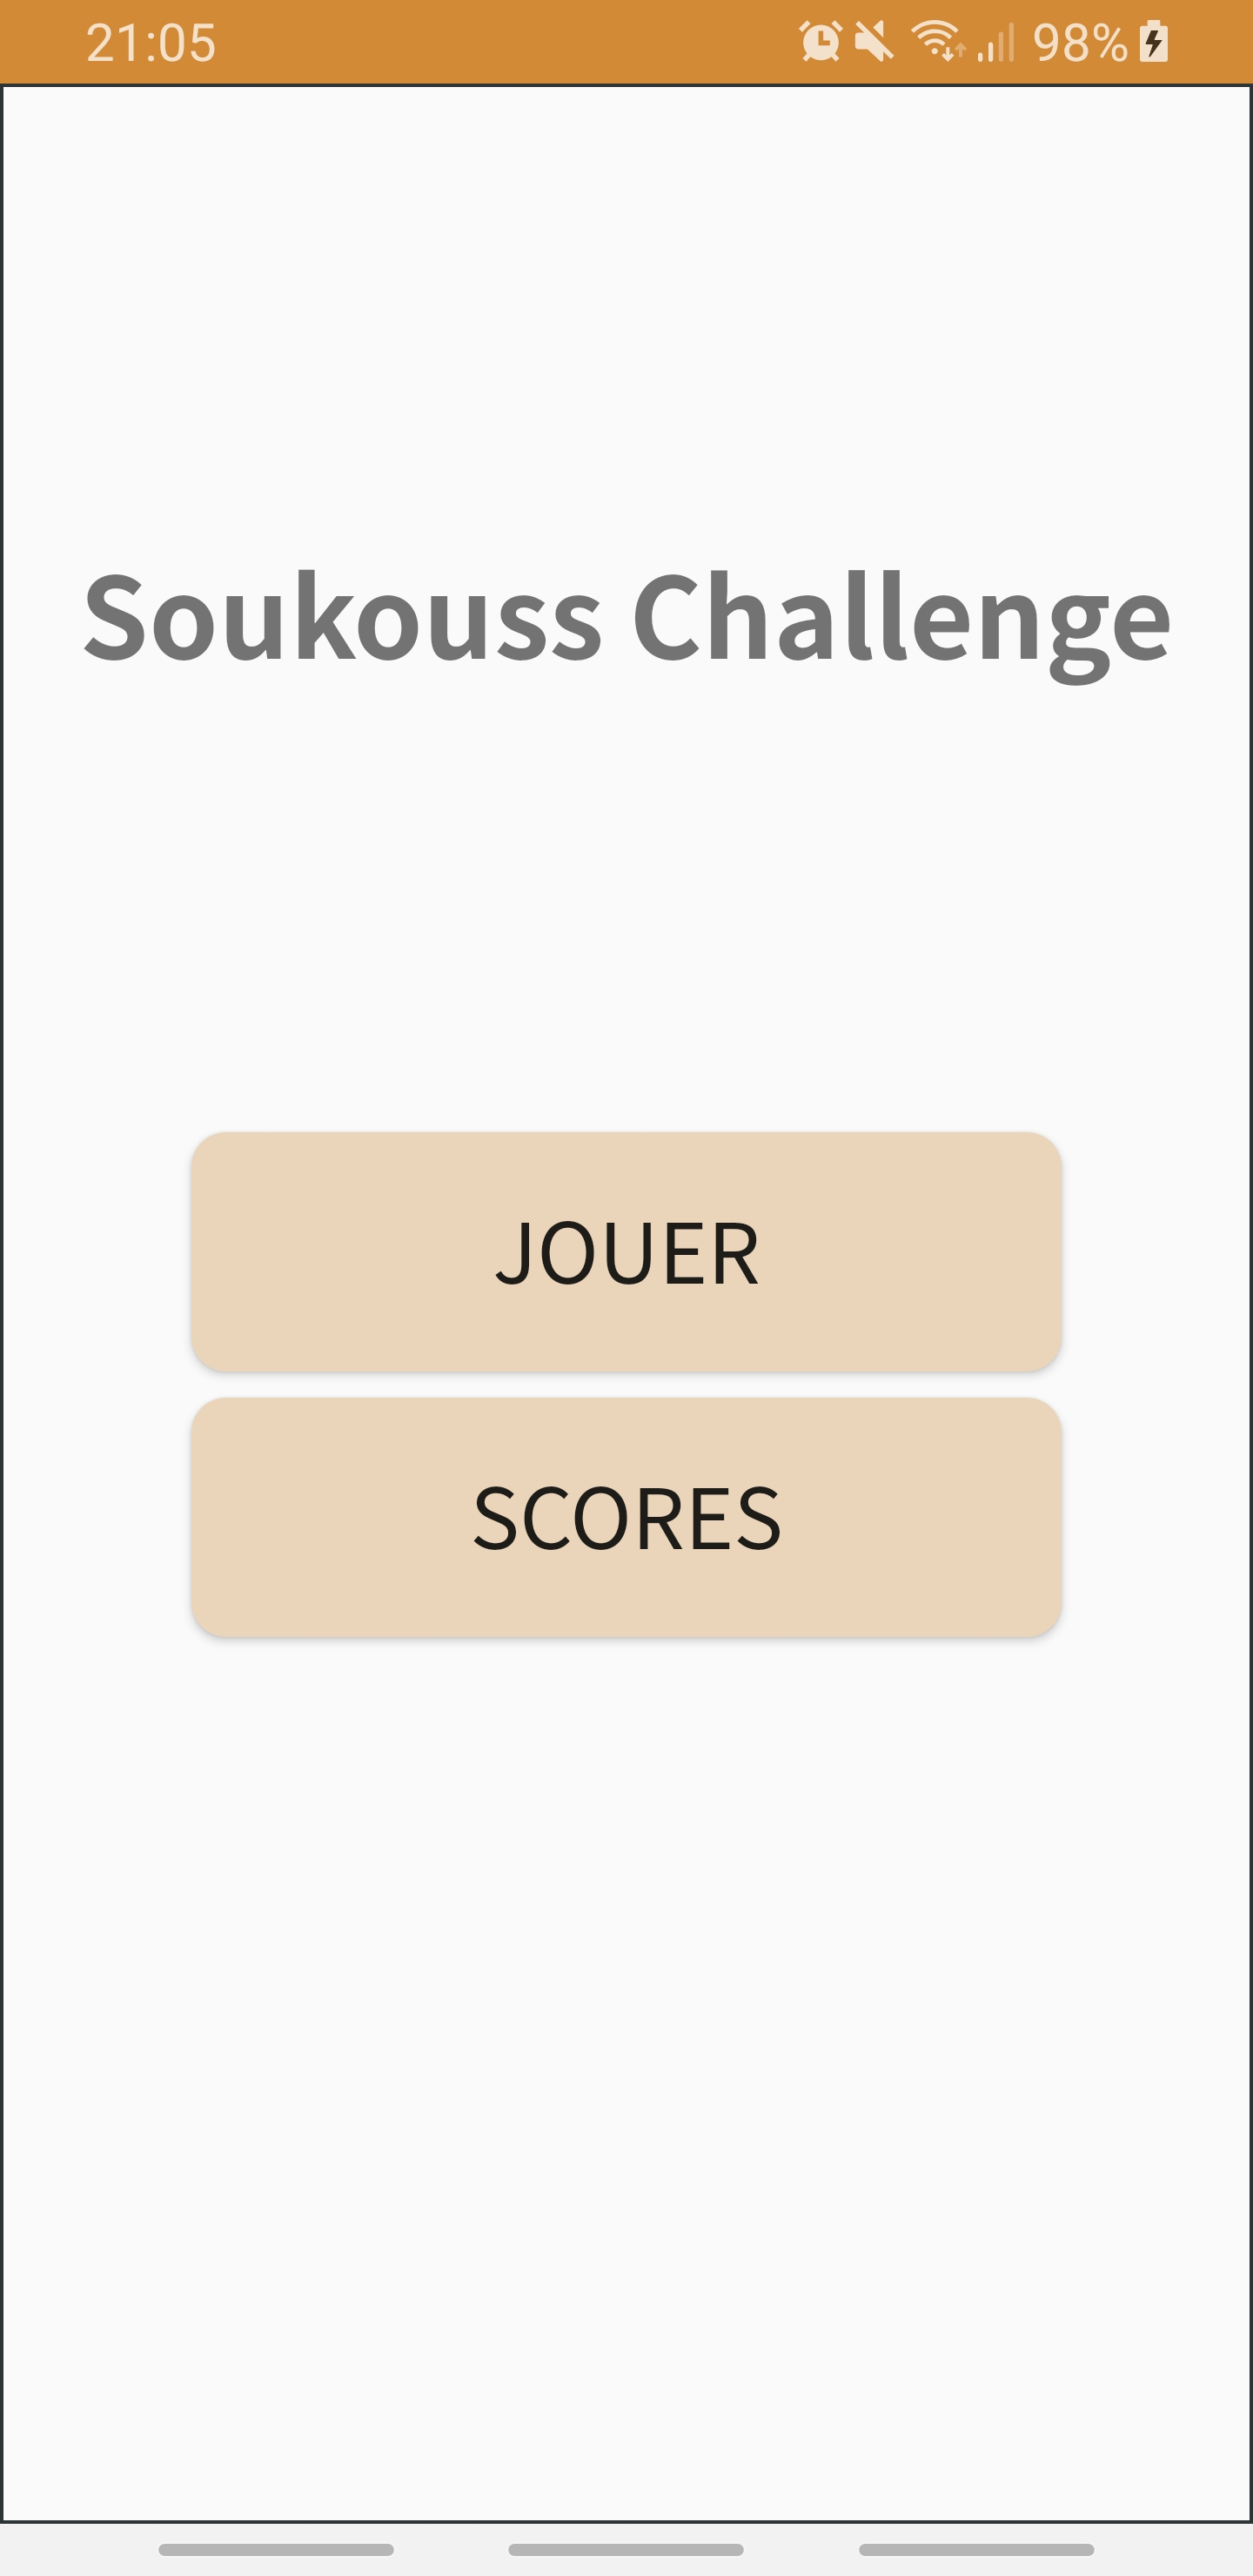
\includegraphics[height=7cm]{Images/VueAccueil.jpg} \end{center}
     \end{column}
     \end{columns}
\end{frame}

\begin{frame}{Description générale de l'application}
    \begin{columns}[T]
    \begin{column}[c]{5cm}
        \begin{center}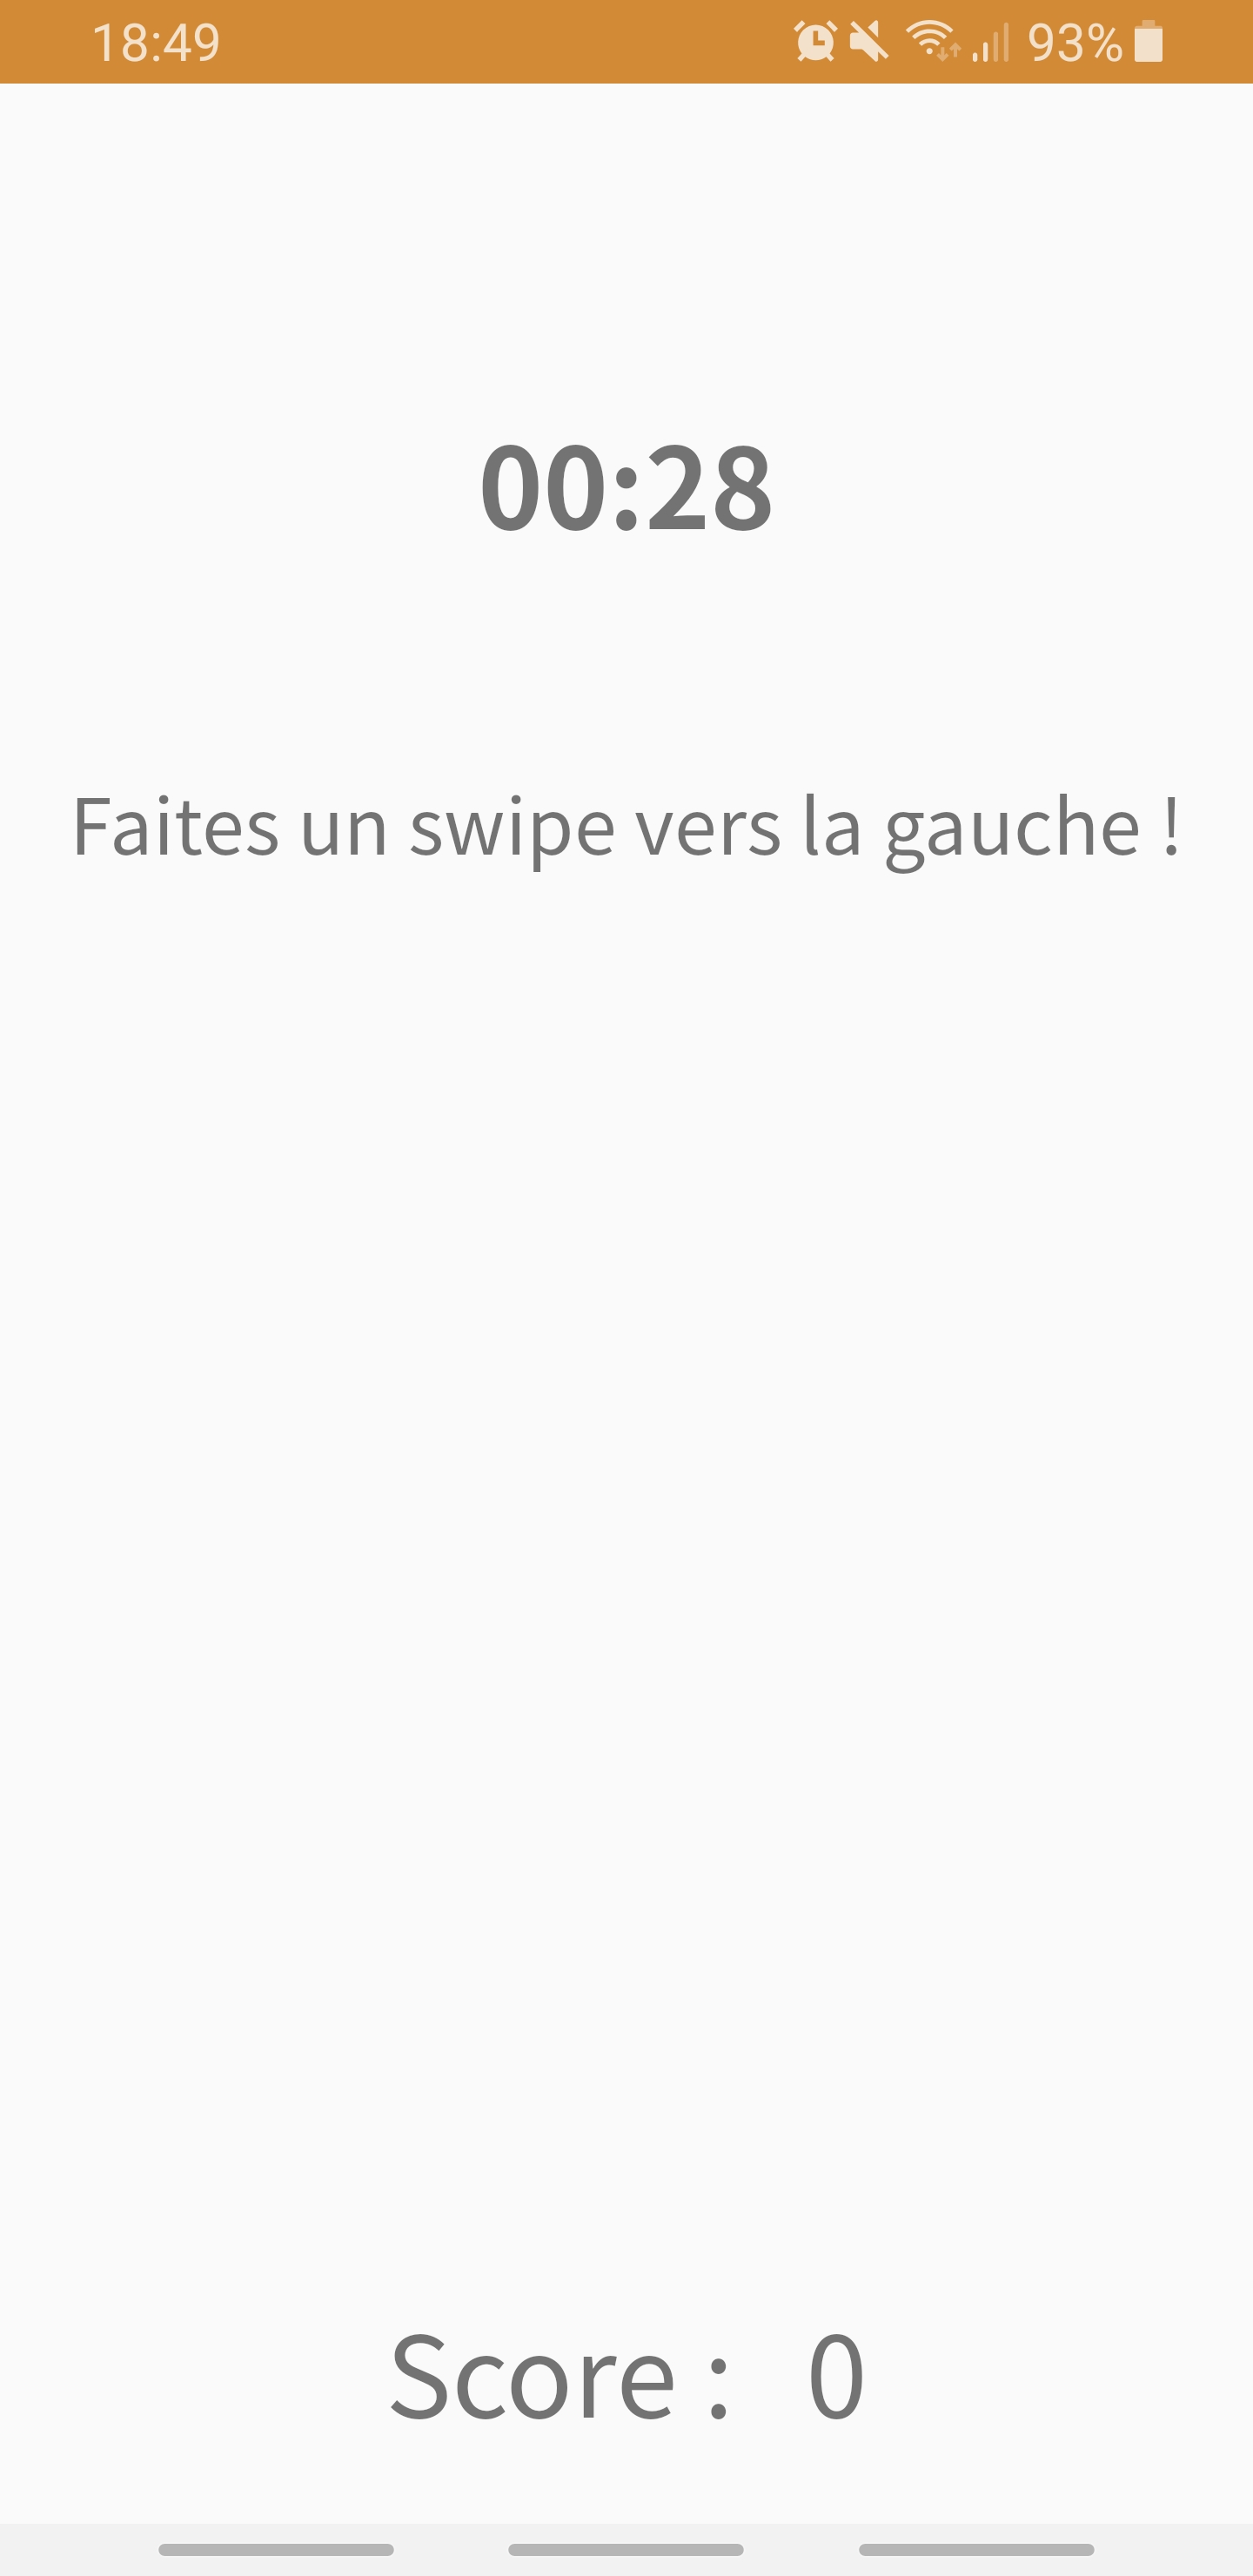
\includegraphics[height=7cm]{Images/VueJeu.jpg}
        \end{center}
    \end{column}
    \begin{column}[c]{5cm}
    \LARGE{La vue de jeu}
    \end{column}
    \end{columns}
\end{frame}

\begin{frame}{Description générale de l'application}
    \begin{center}
        \textbf{\LARGE{Principe du jeu}}
    \end{center}
    \begin{center}
        \begin{columns}[T]
    \begin{column}[c]{5cm}
        \begin{center}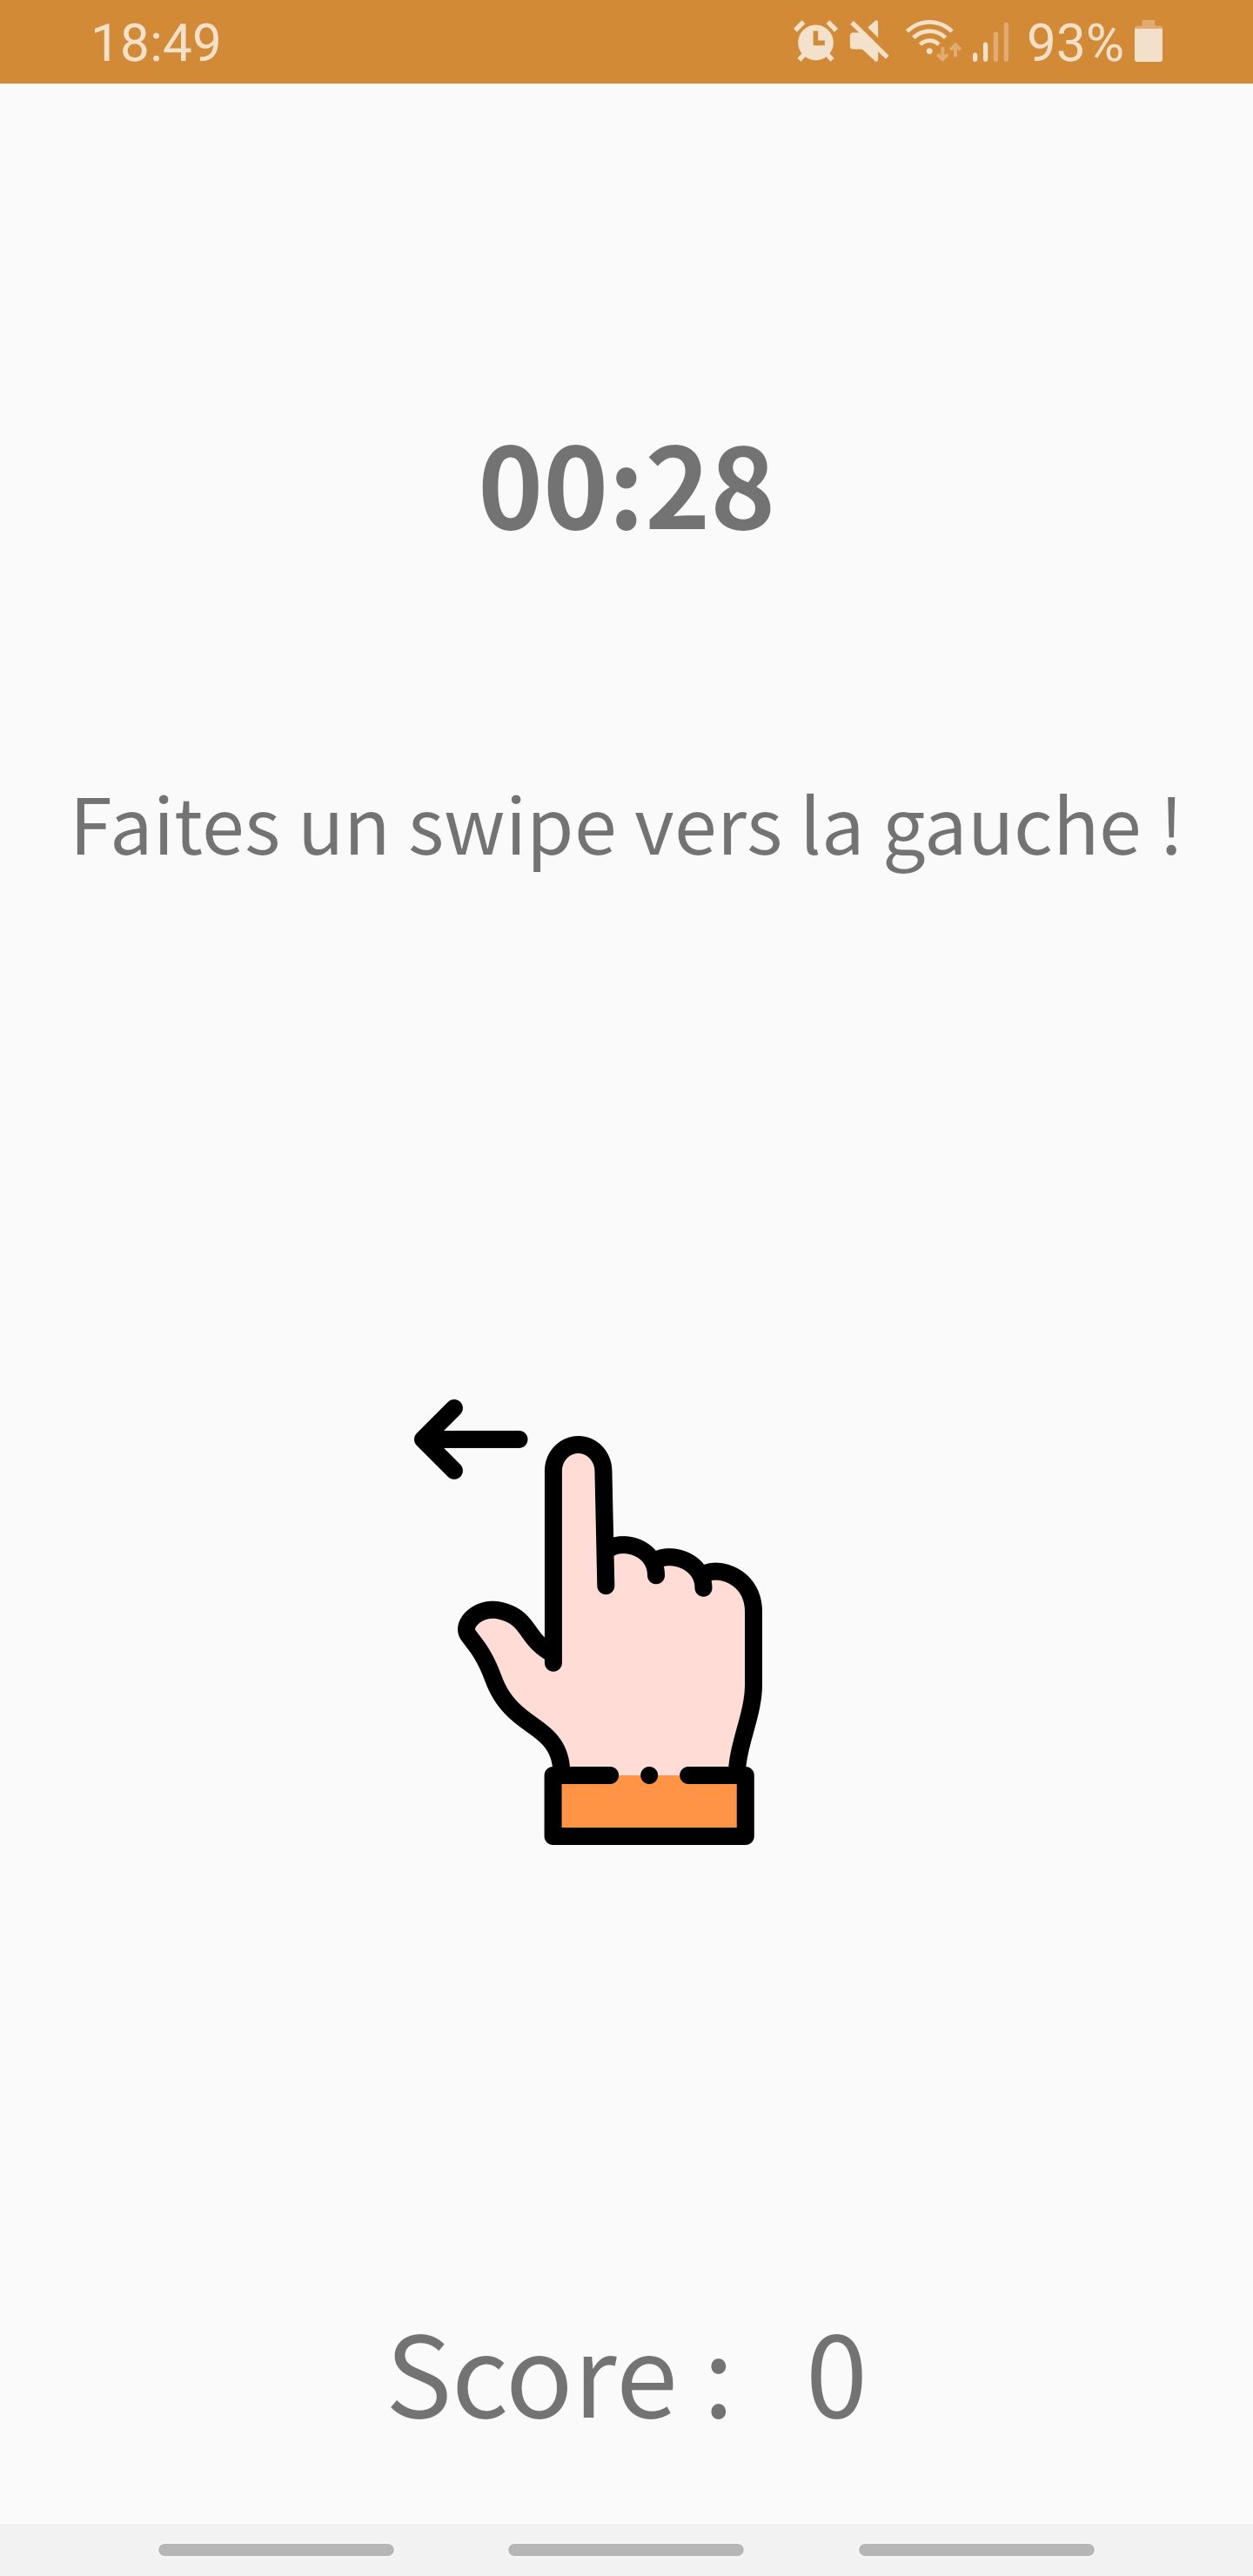
\includegraphics[height=5cm]{Images/game_swipe.png}
        \end{center}
    \end{column}
    \begin{column}[c]{5cm}
        \begin{center}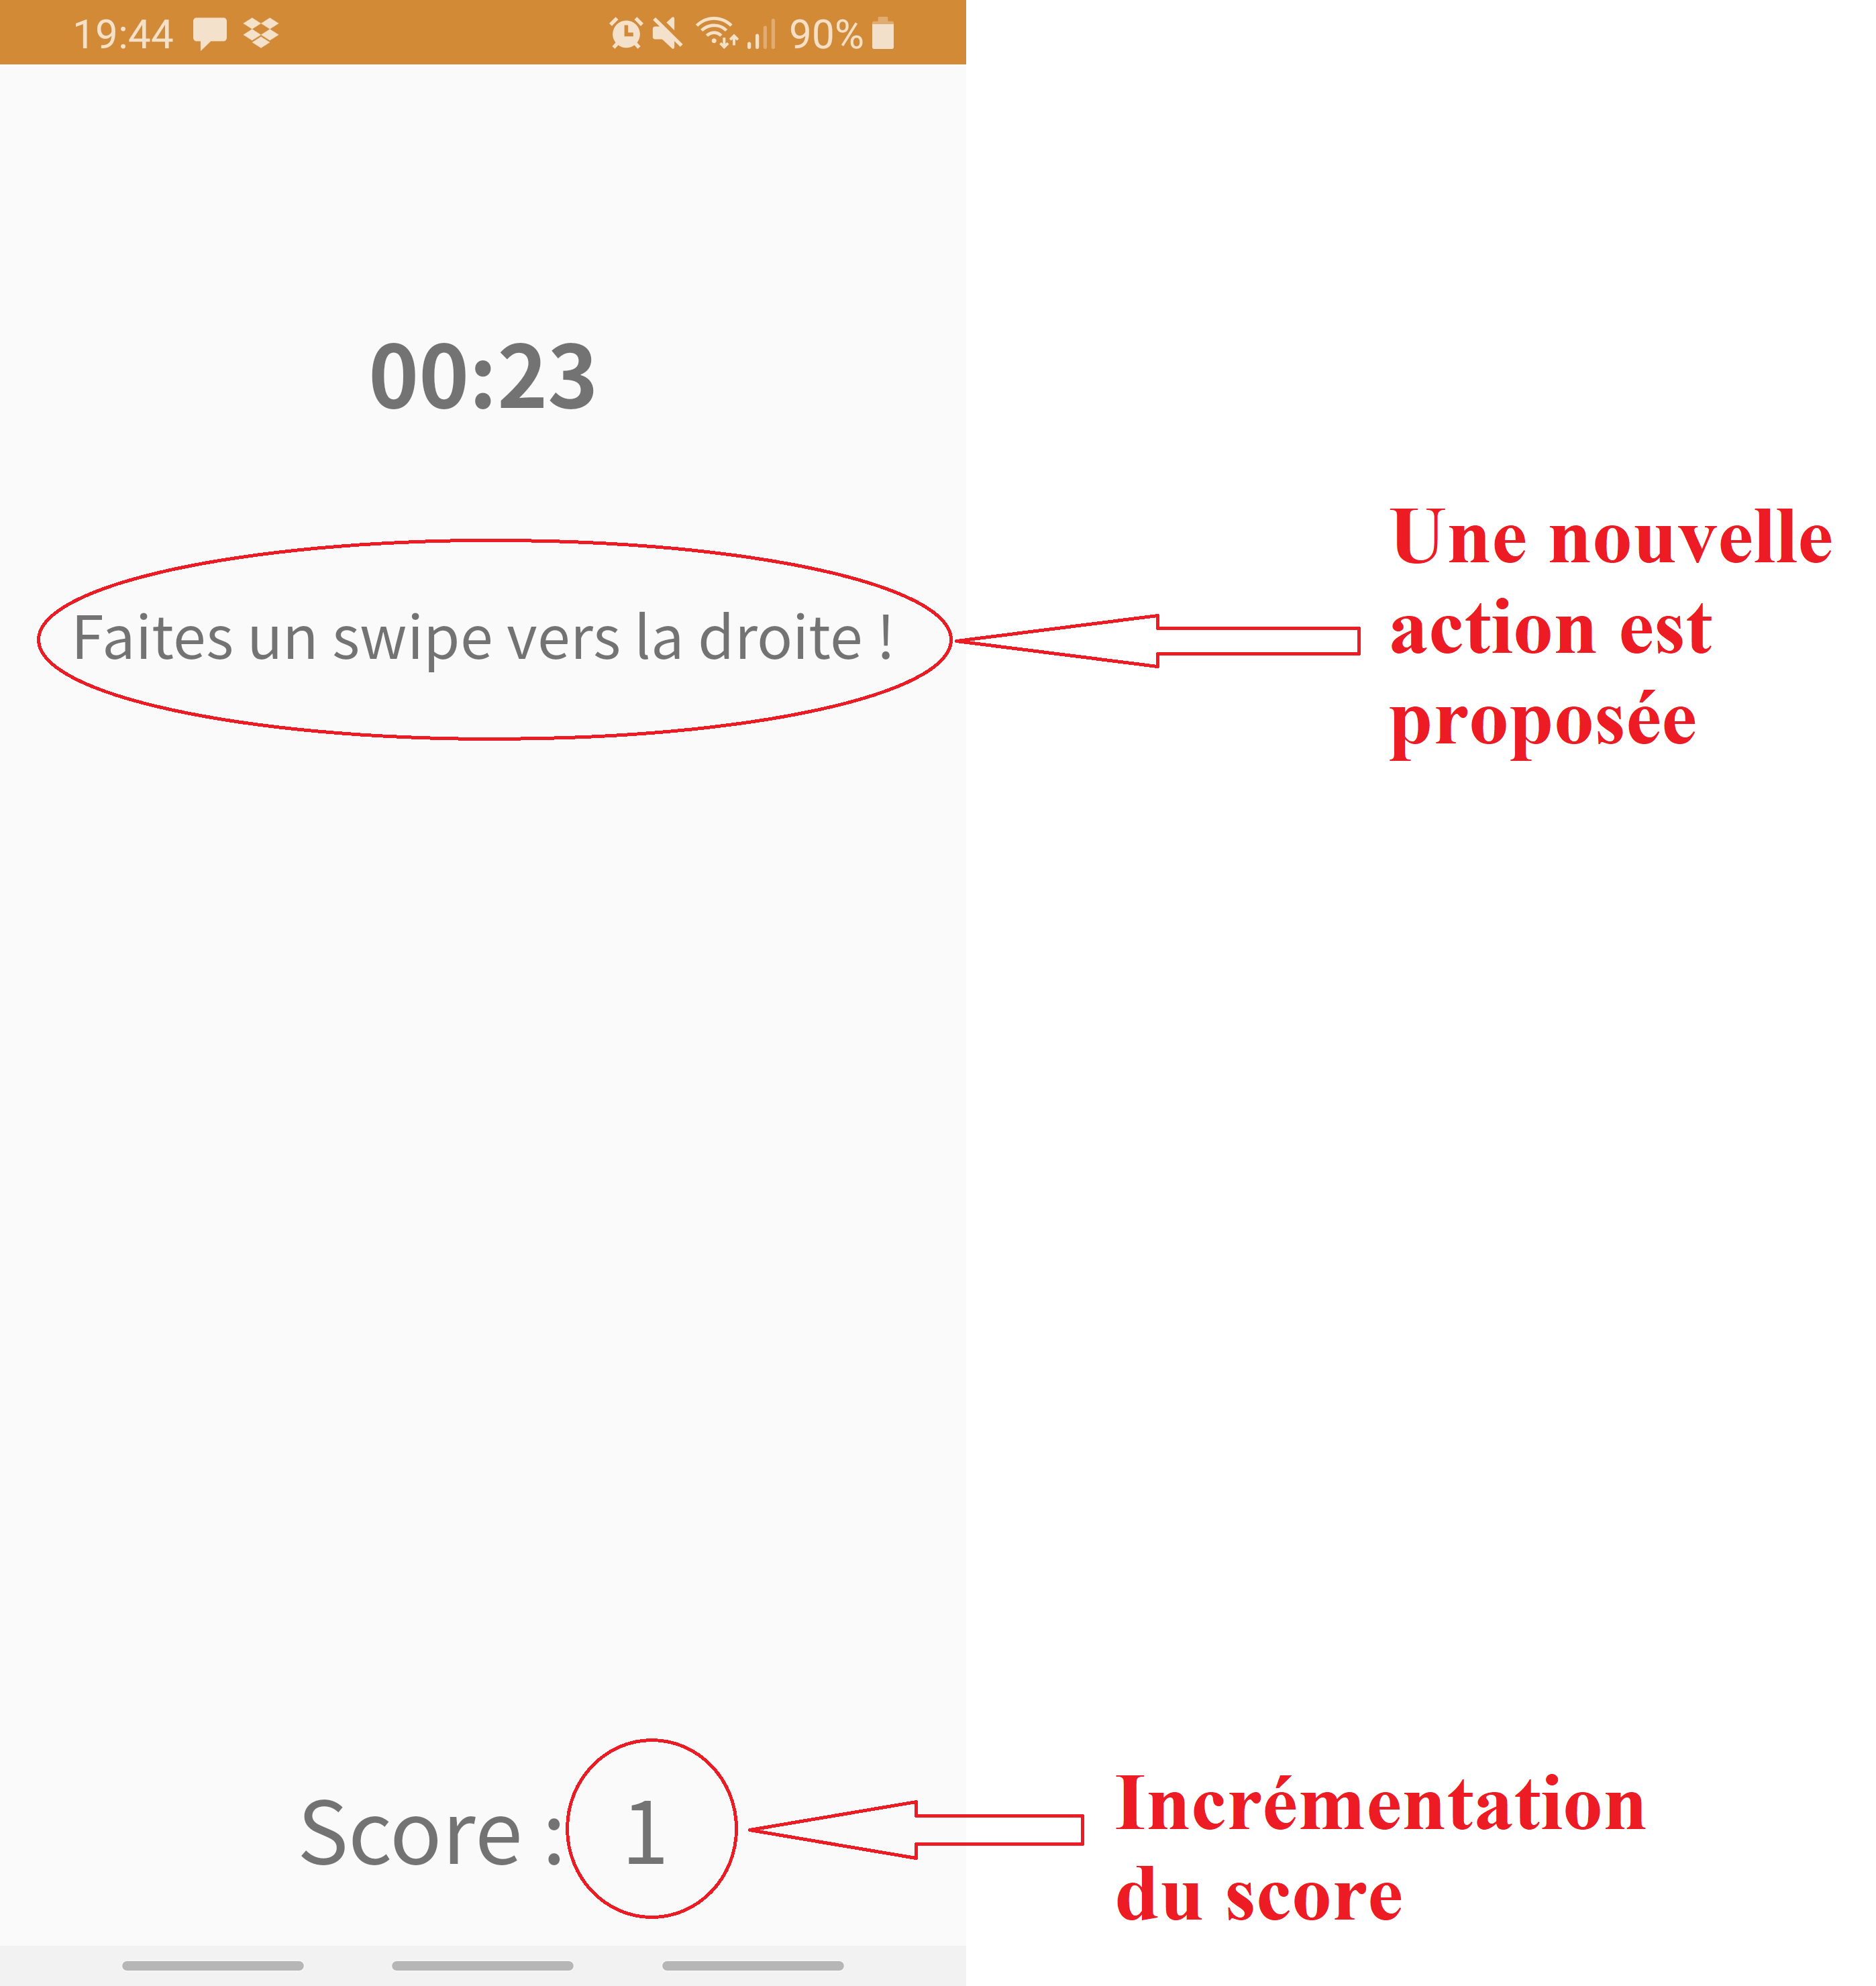
\includegraphics[height=5cm]{Images/legende_jeu.png}
        \end{center}
    \end{column}
    \end{columns}
    \end{center}
\end{frame}

\begin{frame}{Description générale de l'application}
    \begin{columns}[T]
     \begin{column}[c]{5cm}
     \LARGE{Pop-up de fin de jeu}
     \end{column}
     \begin{column}[c]{5cm}
     \begin{center}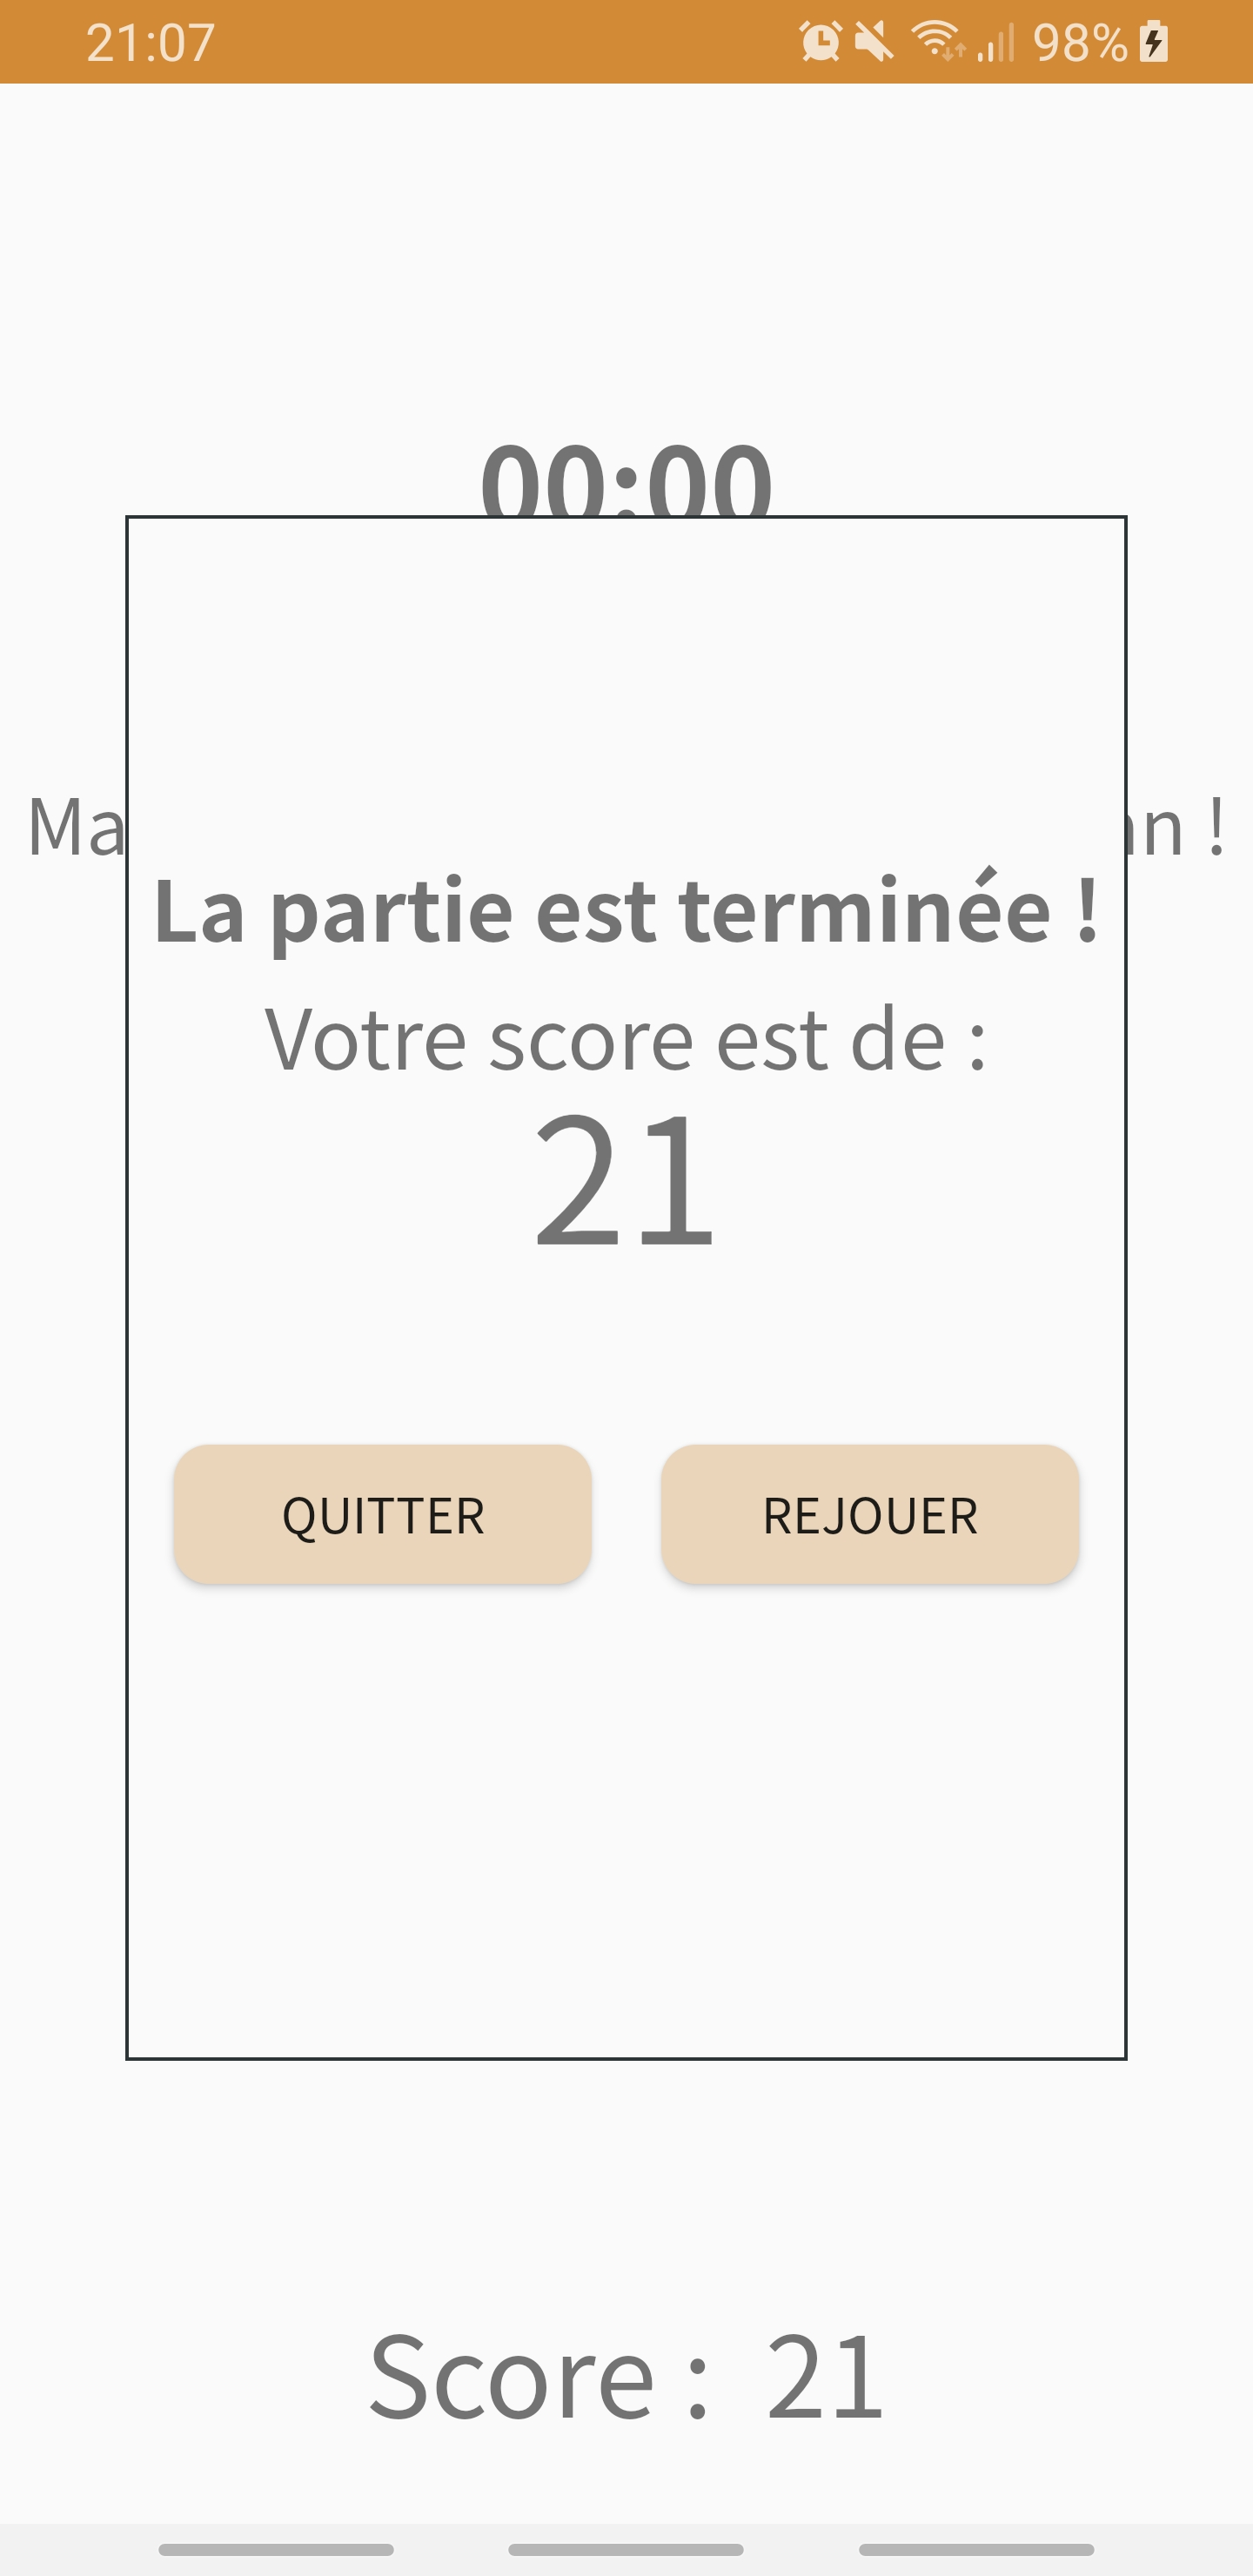
\includegraphics[height=7cm]{Images/PopUpdefin.jpg}
     \end{center}
     \end{column}
     \end{columns}
\end{frame}

\begin{frame}{Description générale de l'application}
    \begin{columns}[T]
    \begin{column}[c]{5cm}
    \begin{center}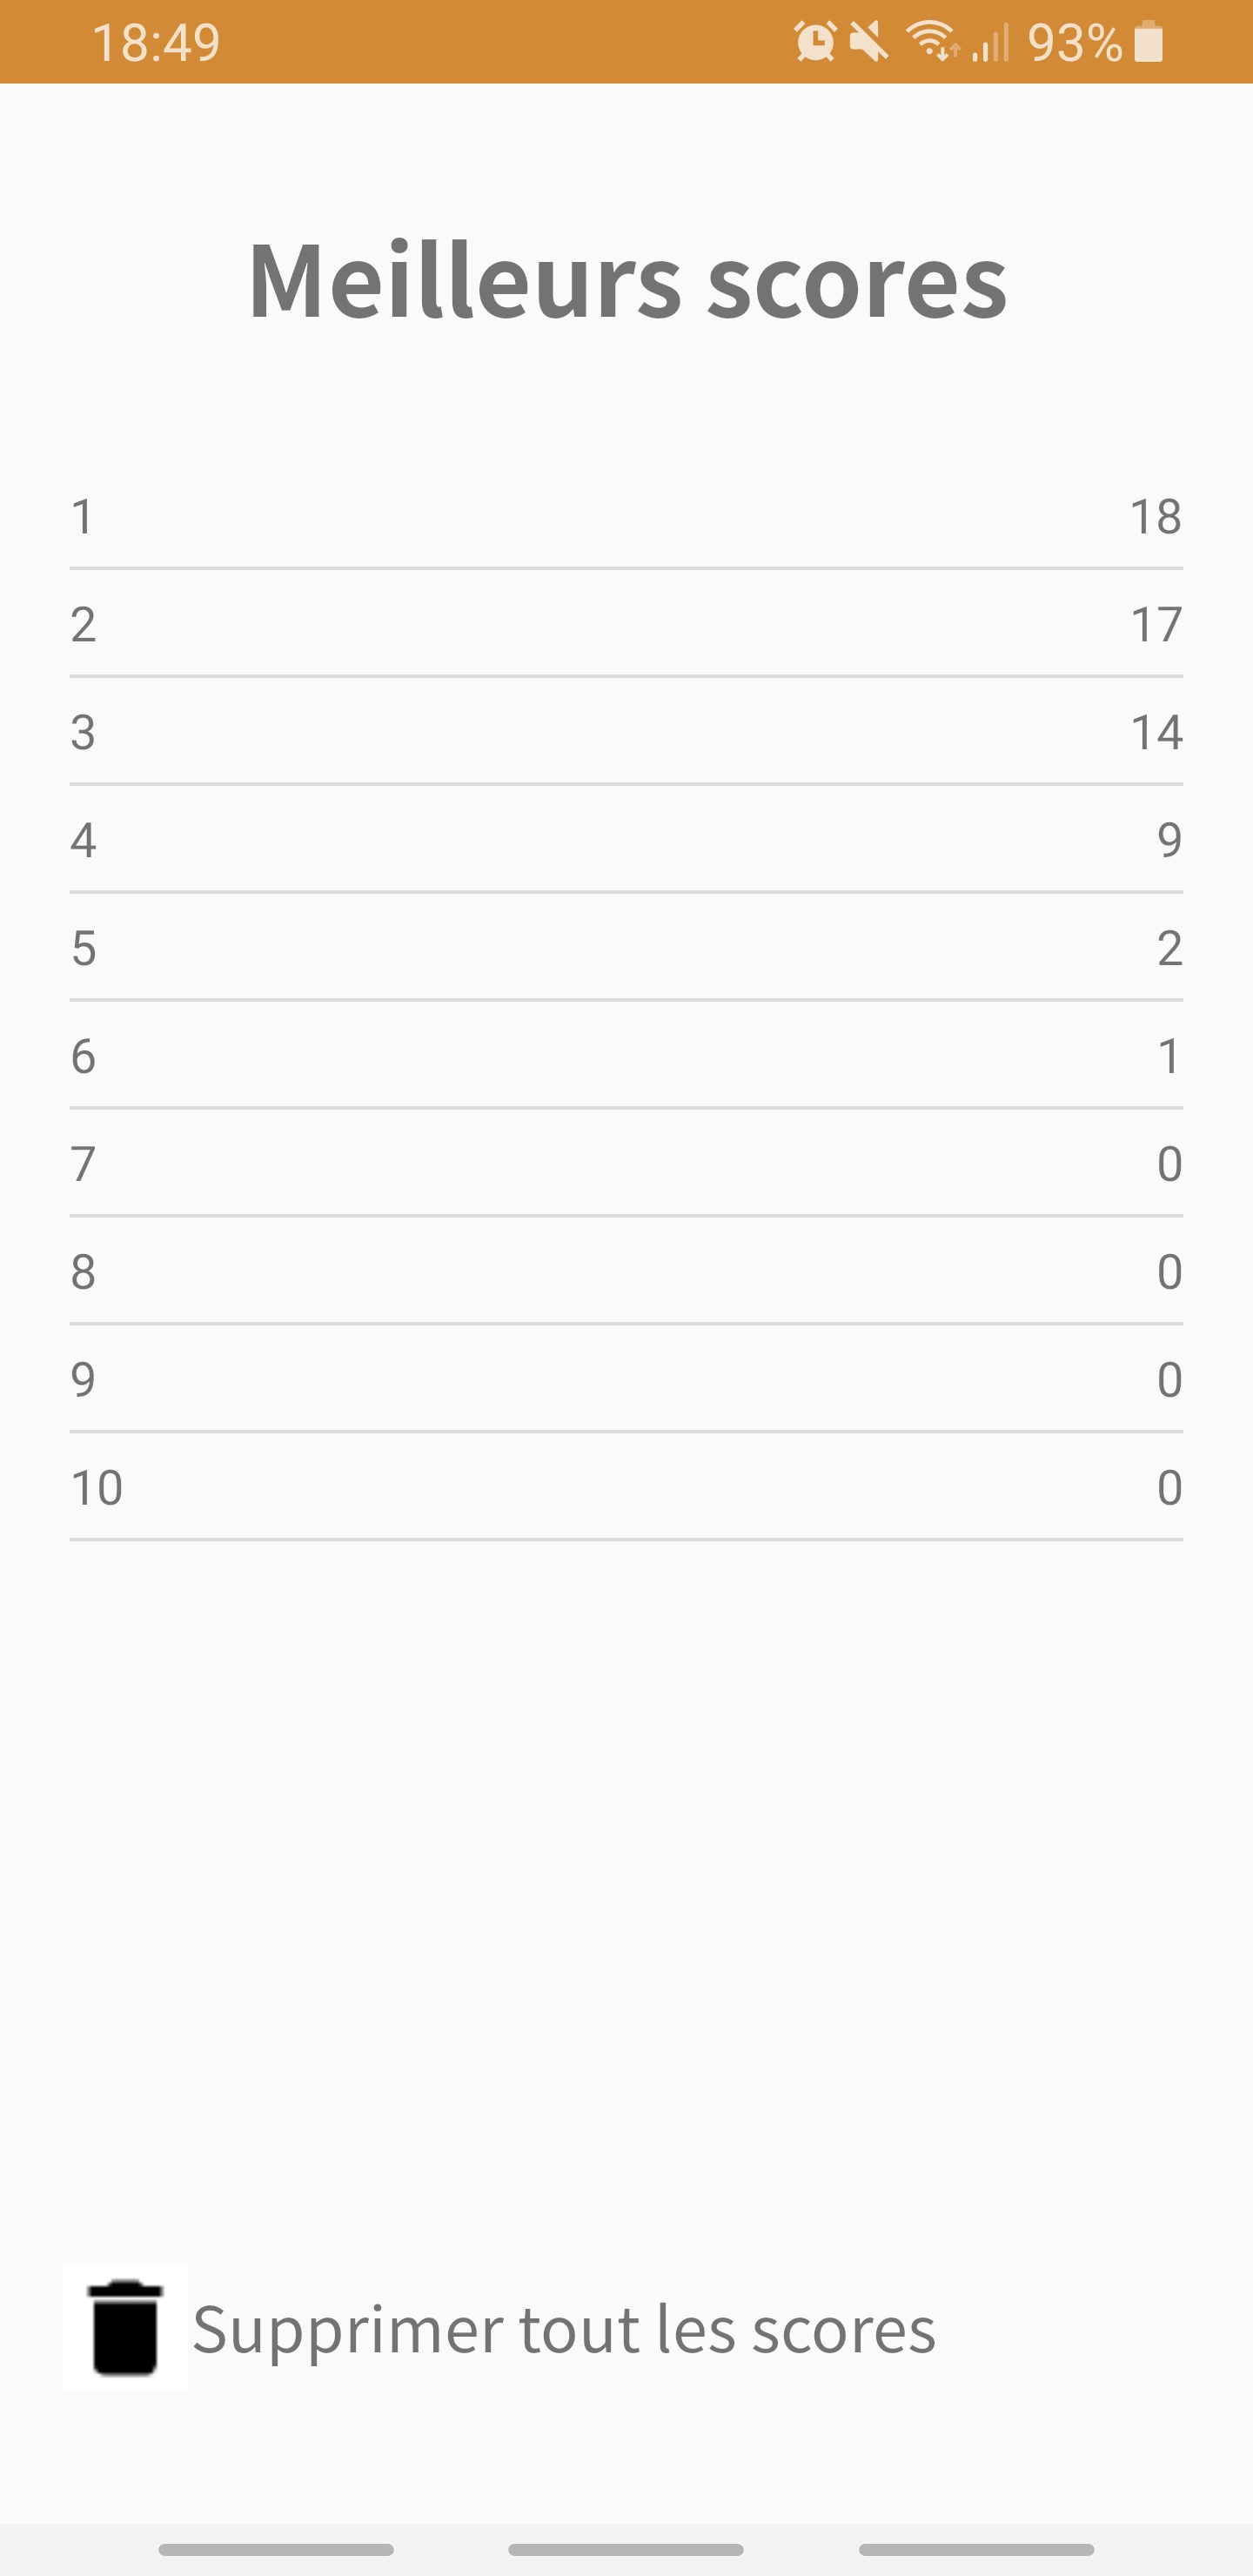
\includegraphics[height=7cm]{Images/VueScores.jpg}
     \end{center}
    \end{column}
    \begin{column}[c]{5cm}
    \begin{center}
        \LARGE{La vue des meilleurs scores}
    \end{center}
    \end{column}
    \end{columns}
\end{frame}

\section{Conclusion}

\begin{frame}{Conclusion}
    \begin{columns}[T]
    \begin{column}[c]{6cm}
        \textbf{Objectifs atteints}
        \begin{itemize}[label=\ding{51}]
            \item Utilisation de l'accéléromètre, des gestes courants et de l'audio
            \item Consigne respectée
        \end{itemize}
        \vspace{3em}
        \textbf{Nouvelles connaissances}
        \begin{itemize}[label=\ding{51}]
            \item Prise en main des fonctionnalités capteurs, gestes courants et audio
        \end{itemize}
    \end{column}
    \begin{column}[c]{6cm}
        \textbf{Travail en équipe}
        \begin{itemize}[label=\ding{51}]
            \item Organisation du travail
            \item Bonne coopération
        \end{itemize}
        \vspace{3em}
        \textbf{Améliorations possibles}
        \begin{itemize}[label=\ding{220}]
            \item Personnalisation de l'interface
            \item Ajout de nouveaux gestes
            \item Ajout d'un mode multijoueur
        \end{itemize}
    \end{column}
    \end{columns}
\end{frame}

\begin{frame}{Conclusion}
    \begin{columns}[T]
    \begin{column}[c]{5cm}
        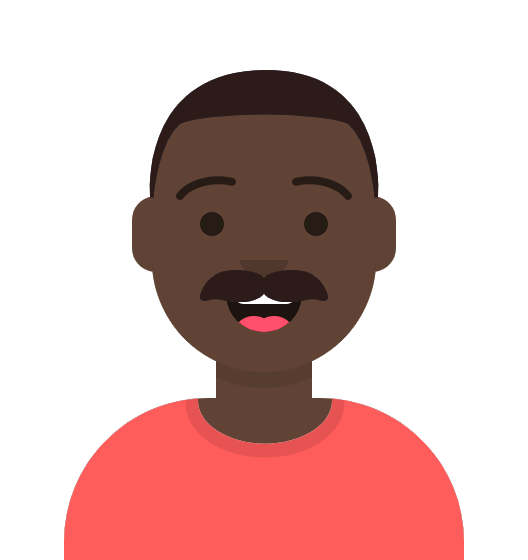
\includegraphics[height=5cm]{Images/avatar_david.png}
    \end{column}
    \begin{column}[c]{5cm}
        
\includegraphics[height=5cm]{Images/avatar_alexandre.png}
    \end{column}
    \end{columns}
    \begin{center}\LARGE{Merci beaucoup de votre attention !}\end{center}
\end{frame}

\section{Démonstration}

\end{document}